\documentclass[12pt]{extarticle}
\usepackage[utf8]{inputenc}
\usepackage{cite}
\usepackage{graphicx}
\usepackage{float}
\usepackage{amsmath}
\graphicspath{ {images/} }

\title{Experiments on Multi-Armed Bandit Problems}
\author{Ajay Subramanian}
\date{May 2019}

\begin{document}

\maketitle

\setcounter{secnumdepth}{0}

\section{Definition of the Problem}
The multi-armed bandit problem is a classic reinforcement learning example wherein pulling each arm of a slot machine rewards us with a stochastic reward $q_*(a)$, generated from an unknown distribution. Our objective is to select the arms one-by-one in a sequence such that we maximise the total reward in the long term. There are some interesting observations that we can make here.

\begin{enumerate}
	\item Bandit problems are a subset of Immediate RL problems in which for every action $a_t$ we receive a corresponding reward $R_t$ with no delay. Also, $R_t$ is a function of only $a_t$ and is independent of any state variables.
	\item A major challenge of solving such problems is handling the exploration-exploitation trade-off. More exploitation maximizes the reward, but only from a a limited action space. Excessive exploration can result in a better estimated reward $Q(a)$ but also increases the regret i.e. payoff lost out on the long term.
I have experimented and analyzed the $\epsilon$-Greedy, Softmax action selection, and UCB-1 algorithms on the 10-armed testbed described in \cite{Sutton1998}
\end{enumerate}

\section{Experiments}

\subsection{$\epsilon$-Greedy}

\paragraph{} The $\epsilon$-Greedy algorithm leaves the explore-exploit decision to a parameter $\epsilon$. Exploiting involves taking the action corresponding to the maximum value of $Q_t(a)$.

\begin{figure}[h]
	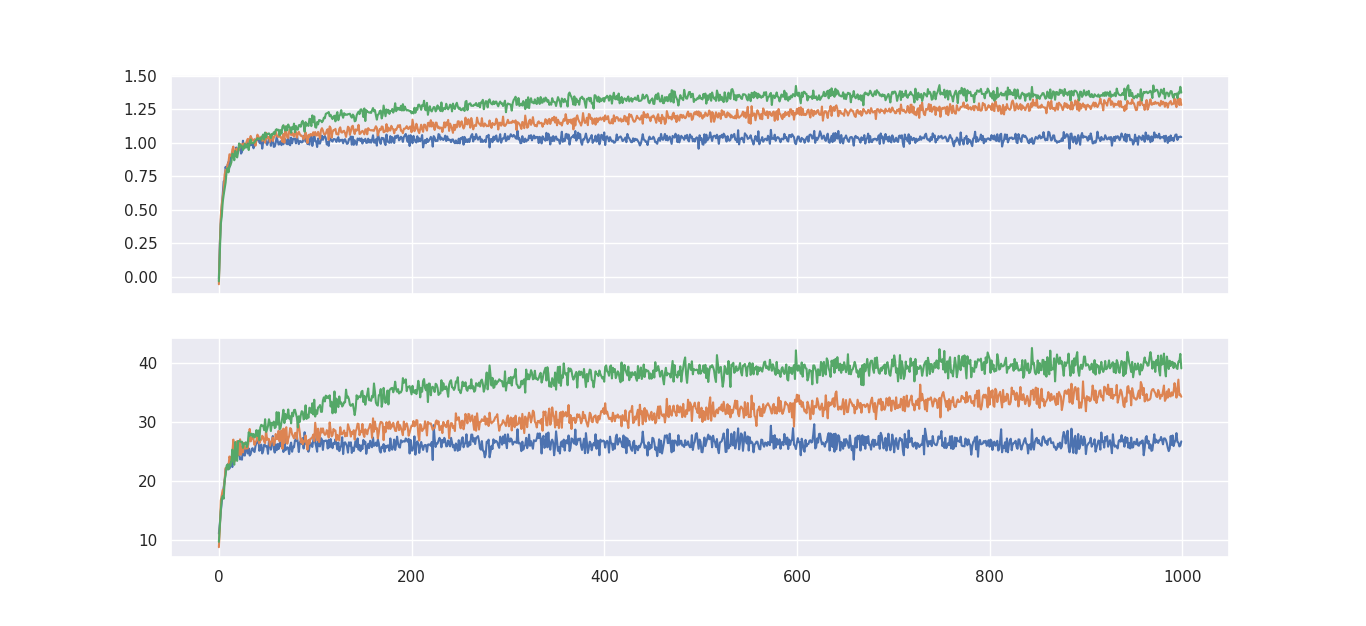
\includegraphics[width=\textwidth, height=10cm]{epsilon-greedy.png}
	\caption{reward vs time (top) and $\%$ optimal action vs time (bottom) for $\epsilon$-greedy for $\epsilon$ taking values 0 (blue), 0.01 (orange), 0.1 (green).}
	\label{fig:epsilon-greedy}
\end{figure}

\paragraph{} As seen in Figure \ref{fig:epsilon-greedy}(top) when the algorithm is set to pure exploitation i.e. $\epsilon = 0$, the reward vs time plot sharply increases on the first trial and then stays almost constant throughout, the reason being that any arm that gives us a positive reward will become the 'optimal' action, following which we will keep pulling that arm. This process is entirely random and hence is not reliable at all. Now, if $\epsilon$ is increased to $0.01$, we expect to take a random action $1\%$ of the time. Due to this, we see a sharp increase, followed by a gradual increase in reward over time. The same trend holds for $\epsilon = 0.1$, but with saturation being reached towards the end. This happens because, with a higher chance of exploration, it becomes easier to find the optimal arm. Hence, the average reward starts becoming more or less constant after timestep ~750. Hence, we see the gap between the $\epsilon=0.01$ and $\epsilon=0.1$ curves decreasing towards the end. This observation could also be explained from the perspective of explore-exploit tradeoffs. Whereas $\epsilon=0.1$ curve identifies the optimum arm faster, but continues to randomize its actions even after that, the $\epsilon=0.01$ plot takes time to figure out the best arm, but almost always pulls that arm once it does.

\paragraph{} The difference between these two is all the more visible in the second plot of Figure \ref{fig:epsilon-greedy} where we see the optimal action being learned by the $\epsilon=0.01$ model gradually over time while it is learned much earlier(at ~400) by $\epsilon=0.01$.

\subsection{Softmax Action Selection}

\begin{figure}[H]
	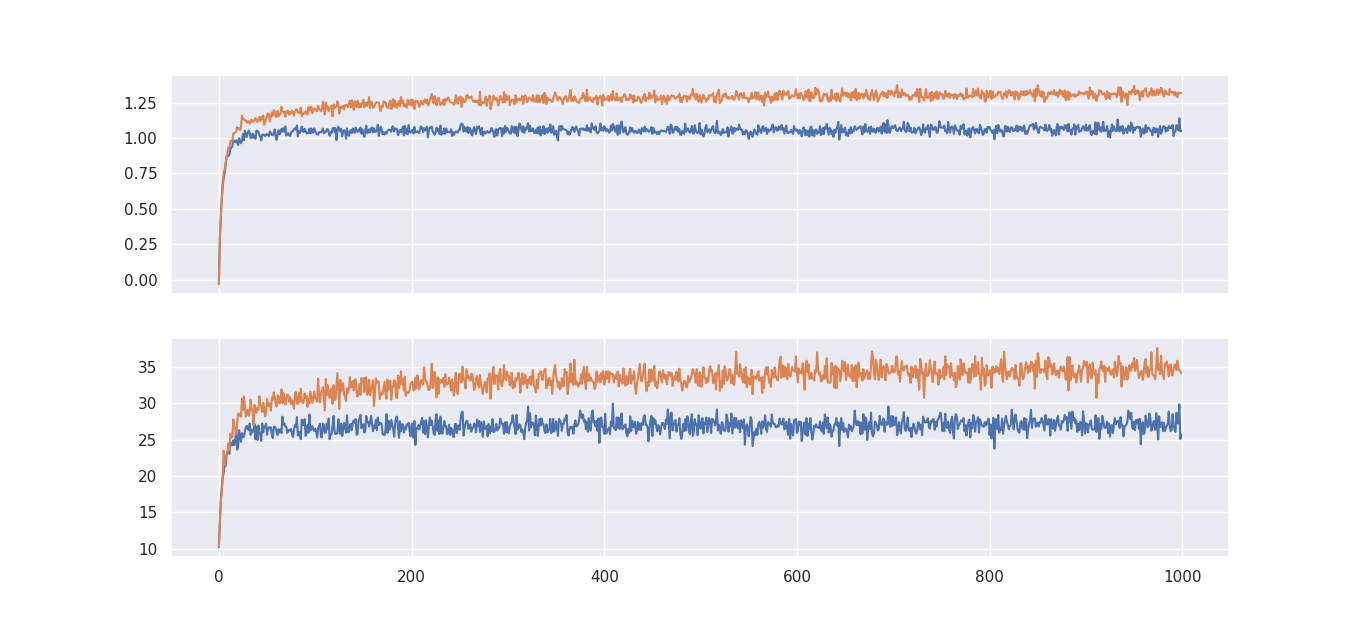
\includegraphics[width=\textwidth, height=10cm]{softmax-action-selection.png}
	\caption{reward vs time (top) and $\%$ optimal action vs time (bottom) for softmax action selection for $\beta$ taking values 0.01 (blue), 0.1 (orange)}
	\label{fig:softmax-action-selection}
\end{figure}

\paragraph{} Using a softmax action selection makes the probability of pulling each arm proportional to its value function $Q_t(a)$. This makes the exploration process more efficient and helps us identify the optimal arms much faster.

\paragraph{} When we compare the curves in Figure \ref{fig:softmax-action-selection} with those in Figure \ref{fig:epsilon-greedy}, we can clearly make out that the optimization of reward occurs much earlier when we use softmax action selection. This is because of the more efficient action selection process. Arms that consistently return a lower reward will have a lower value function i.e. a lower probability of being selected. This is in contrast to the pure $\epsilon$-greedy case where exploring meant giving equal chances to each sub-optimal arm irrespective of how consistently badly or well they have performed.

\paragraph{} We would also like to observe the alteration of the plots when the value of $\beta$ is varied, in this case taking values 0.01 and 0.1. The most important difference is that a higher value of $\beta$ correlates to a more even probability distribution, and therefore more randomness, while a lower $\beta$ value corresponds to more exploitation. These observations are analogous to the differences between $\epsilon$ discussed earlier values and hence similar judgements can be made here too.

\subsection{Upper Confidence Bound (UCB-1)}

\paragraph{} While the two algorithms seen until now aim to achieve Asymptotic Correctness (choosing an arm that gives maximum payoff), the UCB-1 algorithm tries to, in addition, minimize long-term regret i.e. pull least possible number of arms prior to finding the best one. Hence the algorithm goes as follows:

\begin{enumerate}
	\item \textbf{Pull each arm once:} This helps us get early reward estimate of each arm. Asymptotically, pulling each arm atleast once is a necessity to decide the most optimum one.
	\item \textbf{Choose the arm j that maximizes $Q(j) + \sqrt{\frac{2\ln(n)}{n_j}}$:} Before delving deeper into the details, we must understand that UCB works on the principle of 'optimism in the face of uncertainty'. This means that the algorithm aims for an arm better than what is observed from previous data. This is clear in the above expression where the second term can be understood as a confidence interval which shrinks as we pull more arms.
\end{enumerate}

\begin{figure}[H]
	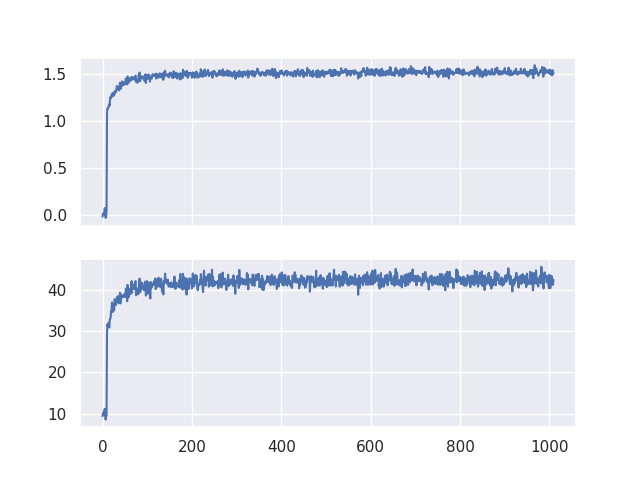
\includegraphics[width=\textwidth, height=10cm]{ucb-1.png}
	\caption{reward vs time (top) and $\%$ optimal action vs time (bottom) for UCB-1}
	\label{fig:ucb-1}
\end{figure}

\paragraph{} It is easily observable from Figure \ref{fig:ucb-1} that UCB-1 achieves the near-optimum action the fastest amongst the three algorithms, on the testbed. A major reason for this is that UCB combines exploration and exploitation within each experiment, thus eliminating the need for a manual transition decision. This is explained as follows. We have already seen the action selection metric.

\begin{equation*}
argmax_j \left(Q(j) + \sqrt{\frac{2\ln(n)}{n_j}}\right)
\end{equation*}

The first term of the expression accounts for exploitation. We know that, in order to maximize our reward and minimize the regret, we have to take an action with a reward in the vicinity of the optimum. Next, at each step, we are willing to test our confidence boundary so that we can better locate the optimum by shrinking the interval. The second term accounts for this exploration attempt. Hence, due to each step of UCB being productive, we can expect it to learn much faster than both $\epsilon$-greedy and softmax, both of which waste some pulls on pure exploration. This hypothesis is clearly visible in Figure \ref{fig:ucb-1}.

\section{Conclusion}
From the detailed analyses of three perspectives at solving bandit problems, we have now a better understanding of the deep intuitions involved in their design. We have also analyzed the role of parameters in the functioning of these algorithms and have learnt the expected behavior of these models with varying parameter values.

\bibliography{cites}
\bibliographystyle{ieeetr}

\end{document}